\chapter{Group Theory}
\myTop{In this chapter we will explain why the \rubik{} can be considered as a group .}
Group theory is a wide subject, containing many different tools and operations.
Here is a general description of group theory along with a way to represent the \rubik{} as a group.
\section{Permutations}
\label{sec:permutations}
%To calculate how many positions the cube can be placed in, we have to look at the general cube terminology in section \ref{sec:generalNotation}
In this section the number of permutations of the \rubik{} will be calculated \cite{rokicki09}. 
The first corner \cpiece{} can be placed in one of eight \cubicle{}s, the next corner \cpiece{} can be placed in one of the seven remaining \cubicle{}s. %, since we already use 1, and so on.% 
This means that the corner \cpiece{}s can be placed in $8\cdot7\cdot6\cdot5\cdot4\cdot3\cdot2\cdot1=8!$ positions. 
%Now the 8 corner \cpiece{}s are placed at the right position. 
This does not mean they have the correct orientation since a corner \cpiece{} has three different \facelet{}s and therefore three different possible orientations. 
This means there are $3^8$ orientations of the eight corner \cpiece{}s, which yields $8!\cdot3^8$ corner permutations. 


The 12 edge \cpiece{}s can be placed in 12 different \cubicle{}s and every edge \cpiece{} can be orientated in two different ways. 
This yields $2^{12}$ different orientations and $12!$ different positions of the edge \cpiece{}s. 
This gives us $2^{12}\cdot12!$ different edge permutations. 

All of these corner and edge permutations adds up to a total of 
\begin{equation*}
3^8\cdot2^{12}\cdot12!\cdot8!=519,024,039,293,878,272,000 \approx 5.2\cdot10^{20} \text{ permutations.}
\end{equation*}
There are however some limitations to a correctly assembled \rubik{}. 
Only seven out of the eight corner \cpiece{}s can be orientated independently. 
The last corner \cpiece{}'s orientation is directly dependent on the other corner \cpiece{}s. 
The same logic applies to the edge \cpiece{}s, which means that only 11 edge \cpiece{}s can be orientated independently.
Furthermore the orientation of the edge \cpiece{}s is also dependent on the orientation of the corners, which halves the number of possible permutations.

The legitimate \rubik{} has 
\begin{equation*}
3^7\cdot2^{10}\cdot12!\cdot8!=43,252,003,274,489,856,000\approx 4.3\cdot10^{19} \text{ permutations.}
\end{equation*}
\section{Definition of the Rubik's Cube Group}
\label{sec:groupDefinition}
To understand how the \rubik{} can be described as a group, it is necessary to understand what a group is.
In group theory the group is written as $(Set, Operator)$ where the set are the elements the group consists of and the operator is the operation that is performed between the elements. When looking at the \rubik{} as a group the set will be a move or a move sequence that is applied to the \rubik{}. The operator in the \rubik{} group will be astrix ($*$) because the \rubik{}s movements are not commutative. The moves are not commutative because it matters in which order they are applied to the \rubik{} \cite[p. 157]{Rubik87}.

To prove that the \rubik{} is a group there are four points it must fulfill:
\begin {enumerate}
\item When two elements are combined with an operation then the new element these create must also be a part of the group. For instance a move \m{M$_1$} and a move \m{M$_2$} then \m{M$_1$} * \m{M$_2$} will form a new move or move sequence which also is a part of the group.

\item $e$ is an empty move (which does not change the configuration of the \rubik{}), if the move \m{M}$* e$ is performed. This means that only the move \m{M} is performed (the move $e$ could be a $360^o$ twist of a face), which means that \m{M}$*e=$ \m{M}.

\item If \m{M} is a move then there is a reverse move, which is called \m{M'}. Therefore \m{M}$*$\m{M} $= e$, which means every element in the group has a reverse move. This holds for the \rubik{} since every move has a reverse, e.g. \m{R} has \m{R'}, and a move sequence can be reversed by first inverting the order and the reverting each move in the sequence.

\item The operation must be associative meaning that the parentheses can be reordered without affecting the result. A move sequence can be defined as the orientation and position it puts each \cpiece{} in. If $c$ is a positioned \cubie{}, \m{M}($c$) will be the \cubicle{} which $c$ ends in after the move is applied. For instance the move \m{R} will move the $ur$ \cubie{} to the $br$ cubicle, so therefore \m{R}$(ur)=br$. If a move sequence is applied, then the operation will look like this \m{B'}$($\m{R}$(ur))=db$.\\
$*$ is associative because (\m{M}$_1*$\m{M}$_2)*$\m{M}$_3$ = \m{M}$_1 *$(\m{M}$_2 *$\m{M}$_3$) for any moves \m{M$_1$}, \m{M$_2$} and \m{M}$_3$. (\m{M}$_1 *$\m{M}$_2$)$*$\m{M}$_3$ and \m{M}$_1 *$(\m{M}$_2 *$\m{M}$_3$) does the same operation to every \cubie{}. This is the same as saying [(\m{M}$_1 *$\m{M}$_2 )*$\m{M}$_3$]$(c)=$ [\m{M}$_1 *$(\m{M}$_2 *$\m{M}$_3$)]$(c)=$ \m{M}$_3$(\m{M}$_2$(\m{M}$_1 (c)$)) for any \cubie{} $c$.
\end {enumerate}

As an extension to the first point some moves will form a new move rather than a move sequence, e.g. \m{R}$*$\m{R} $=$ \m{R2}. This goes for any move sequence only containing moves of the same \face{}.

In fact it is possible to define the \rubik{} only using the following set of moves:
(\m{U D F B L R}) since every other move and move sequence can be made out of these six moves.
This is called the Singmaster notation\cite[p. 7]{Joyner02}, but to make shorter move sequences two of such \twist{}s will be denoted with the letter of the move appended by \m{2}, three of such \twist{}s will be denoted with the letter of the move appended by a prime (\m{'}) as stated in section \ref{sec:moveNotation}.
\section{Subgroup}
\label{sec:subgroup}
%From section \ref{sec:permutations} it is given that there is $3^8\cdot2^{12}\cdot12!\cdot8!$ permutations, but it is not all of these permutations that are possible to do. To make it more easy there will only be looked at some moves of the \rubik{} but only the moves of the down and right faces. To better understand $G$, it can be split up in small pieces.
In this chapter it will be proved that a subset of a group also is a subgroup.
A nonempty subset $H$ of the group $(G,*)$ is called a subgroup of $G$ if $(H,*)$ is a group.

Let $(G,*)$ be a group. A nonempty subset $H$ of $G$ is a subgroup of $(G,*)$ if, for every $a, b \in H$, $a * b^{-1} \in H$.

Proof. First, suppose $H$ is a subgroup. If $b \in H$, then $b^{-1} \in H $since$ (H,*)$ is a group. So, if $a \in H$ as well, then $a * b^{-1} \in H$.

Conversely, suppose that, for every $a, b \in H$, $a * b^{-1} \in H$.

\begin {itemize}
\item First, notice that $*$ is associative since $(G,*)$ is a group.
\item Let $a \in H$. Then, $e = a * a^{-1}$, so $e \in H$.
\item Let $b \in H$. Then $b^{-1} = e * b^{-1} \in H$, so inverse exist in $H$.
\item Let $a, b \in H$. By the previous step, $b^{-1} \in H$, so $a* (b^{-1})^{-1} = a* b \in H$. Thus, $H$ is closed under $*$.
\end {itemize}

Therefore, $(H,*)$ is a group, which means that $H$ is a subgroup of $G$.

%\section{The Symmetric Group}
Instead of just looking at configurations of 8 cubies, the configurations of the cube can be seen as $n$ objects. 
These objects be named $1, 2, . . . , n,$ these names are arbitrary. the arranging of these objects can be seen as
putting them into $n$ slots. If the slots is numberet $1, 2, . . . , n,$ can it be define as a function $\sigma : {1, 2, . . . , n} \rightarrow
{1, 2, . . . , n}$ by letting $\sigma(i)$ be the number put into slot $i$.
\begin{comment}
\subsection{Example} 
Tag the objects $1, 2, 3$ in the order $3 1 2$. So, it corresponds to the function $\sigma: {1, 2, 3} \rightarrow {1, 2, 3}$
defined by $\sigma(1) = 3$,$\sigma(2) = 1$, and $\sigma(3) = 2$.
\end{comment}

Imagine that $x\neq y$. Since a number cannot be in more than one slot, if $x \neq y$, slots x and y must contain
different numbers. That is, $\sigma(x) \neq \sigma(y)$. Therefore, $\sigma$ is one-to-one.

Any number $y \in {1, 2, . . . , n}$ must lie in some slot, say slot x. Then, $\sigma(x) = y$.

But if $\sigma: {1, . . . , n} \rightarrow {1, . . . , n}$ is a bijection, So $\sigma$ can be used to defines the arrangement of the n
objects: just put object $\sigma(i)$ in slot i. So, the arrangements is the same as the set of
bijections ${1, . . . , n} \rightarrow {1, . . . , n}$. Therefore, instead of studying possible arrangements, the bijections can be studied instead.

The Symmetric Group of $n$ letters are the set of bijection from ${1,2,......n}$ to ${1,2,......n}$ with the operation of composition. This group will be called $S_n$
\begin{comment}
\subsection{Exemple}

Let $\sigma,\tau \neq S_3$ be defined as $\sigma(1)=3, \sigma(2)=1, \sigma(3)=2, \tau(1)=1,\tau(2)=3,\tau(3)=2$ so $(\sigma\tau)(1)=\tau(3)=2,(\sigma\tau)(2)=\tau(1)=1, (\sigma\tau)(3)=\tau(2)=3.$
\end{comment}

%\section{Disjoint Cycle Decomposition}
There is a more compact way of writing elements of the symmetric group.
\begin{comment}
\subsection{Example} Consider $\sigma \in S_(12)$ defined by

	$\sigma(1) = 12 \sigma(2) = 4 \sigma(3) = 5 \sigma(4) = 2 \sigma(5) = 6 \sigma(6) = 9
	\sigma(7) = 7 \sigma(8) = 3 \sigma(9) = 10 \sigma(10) = 1 \sigma(11) = 11 \sigma(12) = 8$

We will write $i \rightarrow j$ (i maps to j) to mean $\sigma(i) = j$. Then,

	$1 \rightarrow 12, 12 \rightarrow 8, 8 \rightarrow 3, 3 \rightarrow 5, 5 \rightarrow 6, 6 \rightarrow 9, 9 \rightarrow 10, 10 7\rightarrow 1
	2 \rightarrow 4, 4 \rightarrow 2
	7 \rightarrow 7
	11 \rightarrow 11$


This data tells what $\sigma$ does to each number, so it will define $\sigma$. As shorthand, and write
$\sigma = (1 12 8 3 5 6 9 10) (2 4) (7) (11).$

Here, $(1 12 8 3 5 6 9 10), (2 4), (7), and (10)$ are called cycles. When writing the disjoint cycle decomposition,
the cycles is left out with just one number, so the disjoint cycle decomposition of $\sigma$ is
$\sigma = (1 12 8 3 5 6 9 10) (2 4).$ 
\end{comment}
The difinition of a cycle is if the cycle $(i_1  i_2 ... i_k )$ is the element $\tau \in S_n$ defined by $\tau(i_1 ) = i_2 , \tau(i_2 ) = i_3 , . . . , \tau(i_k  -1) =
i_k , \tau(i_k ) = i_1 $ and $\tau(j) = j$ if $j \neq i_r $ for any $r$. The length of this cycle is $k$, and the support of the cycle
is the set ${i_1 , . . . , i_k }$ of numbers which appear in the cycle. The support is denoted by supp $\tau$ . A cycle of
length $k$ is also called a $k-cycle$.

If two cycles $\sigma$ and $\tau$ are disjoint if they have no numbers in common; that is, supp$\sigma \cap$ 
supp $\tau = \oslash$

Let $\sigma,\tau\in S_n$ be cycles. If $\sigma$ and $\tau$ are disjoint, then $\sigma\tau = \tau\sigma$.

Let $i\in{1, . . . , n}.$ Since $supp \sigma\cap supp \tau = \oslash,$ there are only two possibilities:
\begin{itemize}
\item $i \notin supp \sigma and i \notin supp \tau. In this case, \sigma(i) = i and \tau(i) = i, so (\sigma \circ \tau)(i) =\tau(i) = i and
(\tau \circ \sigma)(i) = \sigma(i) = i.$

\item Otherwise, $i$ is in the support of exactly one of $\sigma$ and $\tau$. it may suppose without loss of generality that
$i \notin supp \sigma$ and $i \in supp \tau.$ Then, $\sigma(i) = i,$ so $(\sigma \circ \tau)(i) = \tau(i).$ On the other hand, $(\tau \circ \sigma)(i) = \sigma(\tau(i)).$
Now, since $\tau(i) \in supp \tau and supp \tau \cap supp \sigma = \oslash, \tau(i) \notin supp \sigma.$ Therefore, $\sigma(\tau(i)) = \tau(i).$ So,
again there is $(\sigma\tau)(i) = (\tau\sigma)(i).$
\end{itemize}

Therefore, $(\sigma \tau)(i) = (\tau \sigma)(i) = i$ for all $i$, which shows that $\sigma \tau= \tau \sigma$.
Any $\sigma \in S_n$ can be written as a product (under the group operation, which is composition) of disjoint cycles.
This product is called the disjoint cycle decomposition of $\sigma.$ In the example, there was given a method for finding
the disjoint cycle decomposition of a permutation.
The identity permutation will be written as $1$.

\begin{comment}
\subsection{Example} $S_2$ consists of two permutations,$ 1 and (1 2).$

\subsection{Example} Let $\sigma, \tau \in S_6$ be defined by

$\sigma(1) = 3 \sigma(2) = 5 \sigma(3) = 4 \sigma(4) = 1 \sigma(5) = 2 \sigma(6) = 6
\tau(1) = 5 \tau(2) = 4 \tau(3) = 3 \tau(4) = 2 \tau(5) = 1 \tau(6) = 6$

In cycle notation, $\sigma = (1 3 4)(2 5)$ and $\tau = (1 5)(2 4)$. Then, $\sigma \tau= (1 3 2) (4 5)$ and $\sigma \tau= (1 2)(3 4 5)$. it
can also easily compute $\sigma^2 = (1 4 3) and \tau^2 = 1.$
\end{comment}
If $\sigma \in S_n$ is the product of disjoint cycles of lengths $n_1, . . . , n_r$ (including its 1-cycles),
then the integers$ n_1, . . . , n_r$ are called the cycle type of $\sigma$.

%\section{Cube Moves keep}

Each move of the \rubik{} will be described by using a slightly modified cycle notation. A description of what happens to each oriented cubie will be needed, so it will describe where each cubie moves and where each face of the cubie moves. For example, if the \rubik{} is unfolded, then draw the down face, so it will look like the following:


\begin{figure}[h]
	\centering	
		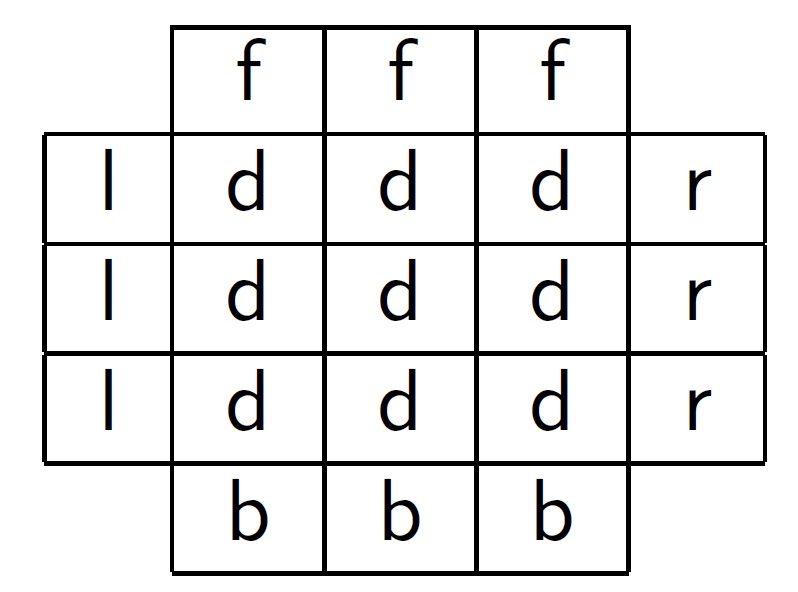
\includegraphics [scale=0.2]{input/pics/rubiks1.jpg}
			\caption{\myCaption{Remember!!}}
	\label{fig:rubiks1}
\end{figure}

Rotate this face clockwise by $90\circ$ (this is called the D move), then the down face looks like:

\begin{figure}[h]
	\centering
		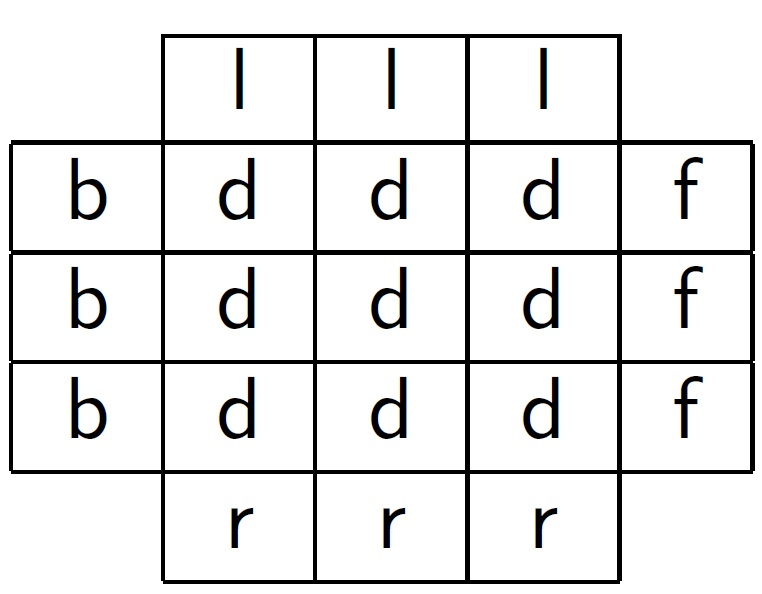
\includegraphics[scale=0.2]{input/pics/rubiks2.jpg}
		\caption{\myCaption{Remember!!}}
	\label{fig:rubiks2}
\end{figure}

So, $D(dlf) = dfr$ because the $dlf$ \cpiece{} now lives in the $dfr$ cubicle (with the down face of the \cpiece{} lying in the down
face of the cubicle, the left face of the \cpiece{} lying in the front face of the cubicle, and the front face of the \cpiece{} lying
in the right face of the cubicle). Similary, $D(dfr) = drb$, $D(drb) = dbl$, and $D(dbl) = dlf$. Do the same thing
for the edge \cpiece{}s, and then $D = (dlf dfr drb dbl)(df dr db dl)$.


\myTail{In this chapter the Rubik's cube has been introduced as a group. Some operations which can be applied to the Rubik's cube group have been explained. It has furthermore been proved that a subset of a group is a subgroup, which means that the same theory that applies to a group also applies to a subgroup.}